
\chapter{Queues}
\label{chap-queue}

A Queue (pronounced by saying the first letter and ignoring all the others) is a data structure which emulates the real word functionality of standing in a line (or queue, for those from Commonwealth nations).  
In a Queue, items are processed in the order they are inserted into the Queue.  So if Alice enters the Queue, followed by Bob, followed by Carla, Alice would be the first to leave the Queue, then Bob, and then Carla.
In other words, the item that has been in the queue the longest is at the front of the Queue and is the next to be processed.


We often refer to a Stack as the LIFO - Last In, First Out - data structure, while the Queue serves as a FIFO - First In, First Out - Data Structure.\footnote{There's gotta be a joke for GIGO - Garbage in Garbage out, to put here.}
The use cases for Queues are fairly obvious.

\section{Queue Operations}
The queue operations are also simple. 

\begin{enumerate}
	\item[\textbf{Enqueue}] Put an item at the back of the Queue.
	\item[\textbf{Dequeue}] Remove and return the item at the front of the Queue.  The next item becomes the new front.
	\item[\textbf{Peek}] Return the front of the Queue, without removing it.
\end{enumerate}


After lists and stacks, this should pose no challenge.
\section{Reference Based Implementation}

Much like the stack in Chapter \ref{chap:stacks}, we can create a queue as an extremely simplified linked list.       

\begin{javacode}{A Reference based Queue}
public class MyQueue<E> {
	// A pedagogical queue
	private Node<E> back;
	private Node<E> front;
	
	private static class Node<E>{
		E item;
		Node<E> next;
		public Node(E item) {
			this.item = item;
		}
	}
	
	public void enqueue(E item){
		Node<E> newBack =  new Node<E>(item);
		back.next = newBack;
		back =  newBack;
	}
	
	public E dequeue() {
		E toReturn =  front.item;
		front = front.next;
		return toReturn;
	}
	
	public E peek() {
		return front.item;
	}
}

\end{javacode}



\begin{pycode}{A Reference based Queue}
class Stack:
	class Node:
		def __init__(self, item):
			self.item = item
			self.next = None

	def __init__(self):
		self.top = None

	def isEmpty(self):
		return self.top is None
	
	def peek(self):
		return self.top.item
	
	def pop(self):
		toReturn = self.top.item
		self.top = self.top.next
		return toReturn
	
	def push(self, item):
		newTop = self.Node(item)
		newTop.next = self.top
		self.top = newTop
\end{pycode}




\section{Array Based Implementation}
Referenced based implementations, but arrays can be slightly more efficient for a number of reasons:



\begin{itemize}
	\item No overhead from references.
	\item foo
	\item Caching - This gets into a bit more optimization we typically concern outselves with, but cpus can cahe the array leading to better performance.  (Can't include until I find a strong citation for this and not being a thing linked lists can do)

\end{itemize}

\section{Built-in Queues}
\subsection{Java's Implementation}

\subsubsection{The \texttt{Queue} - Use on Exams and Psuedocode}
In Java, a \texttt{Queue} is an Interface with the following methods

\begin{description}
	\item[\texttt{offer(item)}] - Java's enqueue.
	\item[\texttt{poll()}] - Java's dequeue.
	\item[\texttt{peek()}] - Java's peek.  A peak name.
\end{description}

In the case of the method call failing, the method will return \texttt{false} or \texttt{null} as applicable.  The Queue interface also provides a version of each the methods that do the exact same thing, but throw an exception instead.  These methods are \texttt{add(item)}, \texttt{remove()}, and \texttt{element()} respectively. 



\begin{figure}
	\centering
	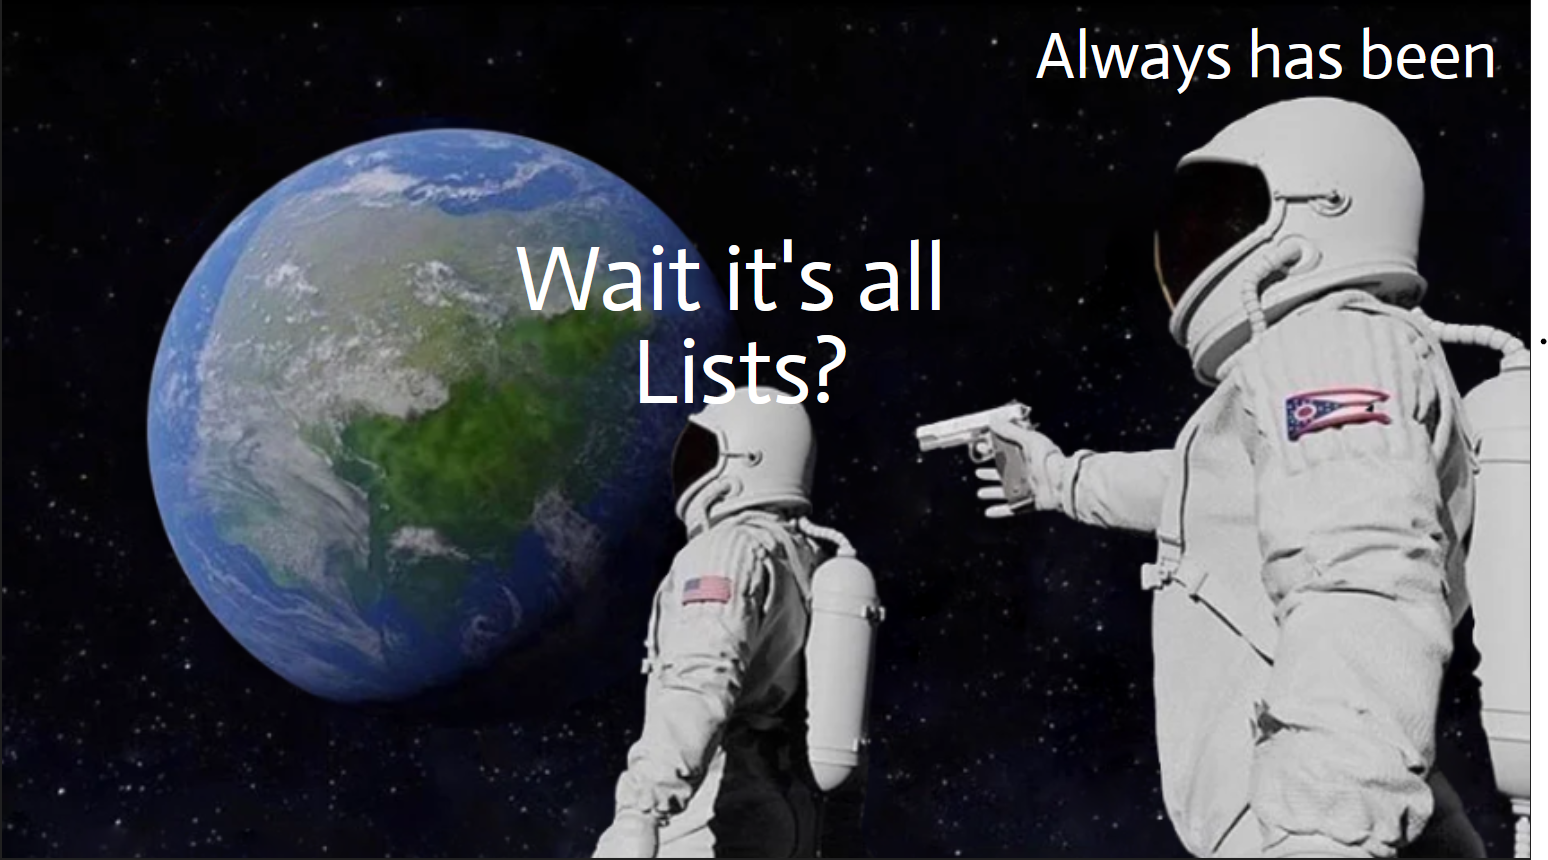
\includegraphics[width=\linewidth]{pics/waitQueuesAreLists}
	\caption{You, after learning about how to do stacks and queues.}
	\label{fig:waitqueuesarelists}
\end{figure}

\subsubsection{The \texttt{Deque} - What You Should Actually Use}

\subsection{Python's Implementation}


\subsubsection{The List as a Queue}

This is your Queue: \texttt{[]}.  Exciting and super foreign, yes?
We can manipulate the list to use it as a Queue like so:

\begin{pycode}{This is bad}
q = []
q.append('a')
q.append('b')
q.append('c') # append to enqueue
q.pop(0)      # you can pop index 0 to dequeue
\end{pycode}

However, a keen reader might remember what we know about python's lists and realize that while the enqueue is fast at $O(1)$ time, the dequeue will be $O(n)$ as all the items need to shift to the left.  

%TODO put in proper citation as opposed to the hyperlink
\href{https://docs.python.org/3/tutorial/datastructures.html#using-lists-as-queues}{In fact, our python documentation explicitly says so:}

\begin{quotation}
It is also possible to use a list as a queue, where the first element added is the first element retrieved (``first-in, first-out''); however, lists are not efficient for this purpose. While appends and pops from the end of list are fast, doing inserts or pops from the beginning of a list is slow (because all of the other elements have to be shifted by one).

To implement a queue, use \texttt{collections.deque} which was designed to have fast appends and pops from both ends. For example:
\end{quotation}


Here's their example on how to use that:
\begin{pycode}{Example deque usage adapted from the python docs}
from collections import deque
queue = deque(["Eric", "John", "Michael"])
queue.append("Terry")           # Terry arrives
queue.append("Graham")          # Graham arrives
queue.popleft()                 # The first to arrive now leaves
								# Yields 'Eric'
queue.popleft()                 # The second to arrive now leaves
                                # Yields 'John'
print(queue)                           # Remaining queue in order of arrival
deque(['Michael', 'Terry', 'Graham'])
\end{pycode}


\subsubsection{The queue package}
